\chapter{Methodology}
\label{ch:methodology}

This project explores the possibility of developing an RFID location sensing system using cost-effective hardware. This chapter gives the reader a detailed overview of the system components and approach to the problem. Section \ref{sec:hardset} presents the hardware setup of the system. Section \ref{sec:probdef} describes the problem this project is trying to solve. Then, the overall software architecture is discussed in section \ref{sec:softarch}. Section \ref{sec:rssitodist} details the methods for converting RSSI to distance measurements. Finally, section \ref{sec:trilatmeth} describes trilateration, a mathematical technique that computes the relative position of an unknown object to three reference objects.

\section{Hardware Setup}
\label{sec:hardset}

The devices used in this project were connected together to form the hardware setup of the system. These components and their specifications are described in detail in section \ref{sec:projhard}. Figure \ref{fig:hardset} is a diagram illustrating how the hardware devices were attached to each other.

\begin{figure}[h]
	\begin{center}
		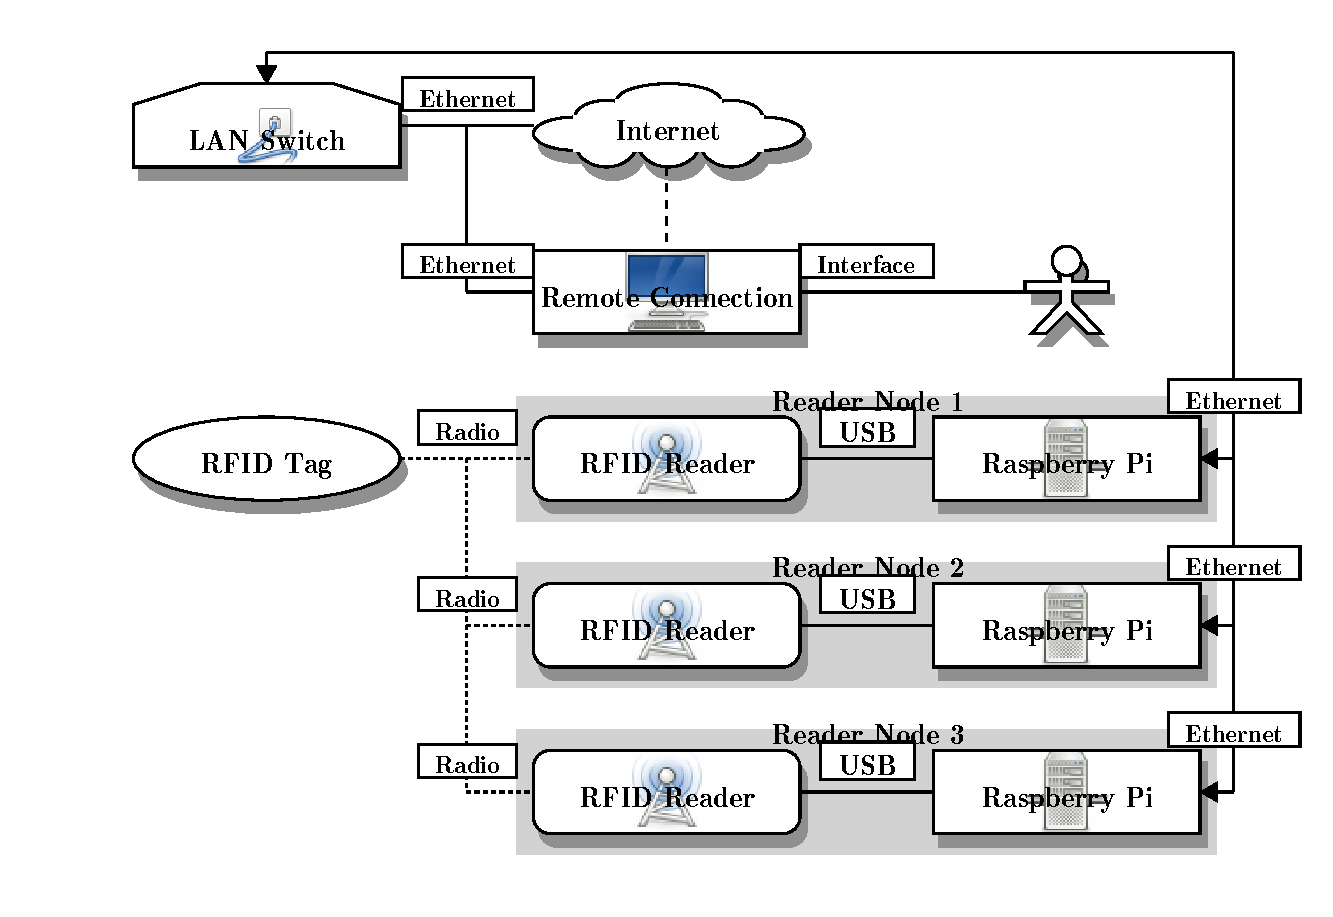
\includegraphics[width=1\textwidth]{figures/blockdiag/hardwaredesign}
		\caption{Hardware setup of the project.}
		\label{fig:hardset}
	\end{center}
\end{figure}

\subsection{Reader nodes}

The building blocks of the system are the reader nodes. Each consists of an RFID reader connected to a Raspberry Pi using USB. The project plan had provisioned extra time to account for the possible complications when interfacing between serial devices and single-board computers. The Raspberry Pis have USB ports that cannot power all kinds of USB devices. Another issue was whether the computers were capable of recognising and communicating with these specific RFID readers. Fortunately, these potential problems did not occur during this project. The RFID devices read identification data from the RFID tag over the air.

\subsection{Computer Network}

The Raspberry Pis were connected in a local area computer network (LAN) using Ethernet cables and a network switch. This allowed them to communicate readings to each other. The Raspberry Pi network provided means for remotely accessing, programming, and controlling the reader nodes. Remote access was established by connecting to the network using the network switch or through a wide area network, such as the Internet.


\subsection{Alternative connectivity using Wi-Fi}

During the project planning phase, an alternative connectivity method was considered. The Raspberry Pis have two USB ports. One of them was occupied by a RFID reader. The spare one could have been used for a wireless network adapter. Then, all reader nodes could connect to a wireless router or form an ad hoc network in order to communicate measurements. This way all Ethernet cabling and the network switch are not required giving a greater flexibility when positioning the reader nodes. Figure \ref{fig:hardsetwifi} in Appendix \ref{sec:hardsetwifi} shows this alternative hardware setup.

There are two matters that complicate this choice of connectivity. First, there is a high probability that the power fed to the USB ports is not enough to supply both an RFID reader and a Wi-Fi adapter. In which case, three powered USB hubs were needed to be purchased. Second, the Raspberry Pis have integrated Ethernet ports. Buying three wireless USB dongles is an unjustifiable expense in case these might not get powered by the single-board computers.

\section{Problem Definition}
\label{sec:probdef}

Given the hardware setup of the system consisting of three reader nodes connected into a computer network, the problem it is trying to solve is to estimate the relative position of an RFID tag to three RFID readers. The system should accept the following inputs:
\begin{itemize}
	\item identification information received from the RFID tag,
	\item RSSI measurements computed at the RFID readers,
	\item and positions of the reader nodes in three dimensions.
\end{itemize}
The system should output the location of the RFID tag relative to the reader nodes. The system should be able to estimate the tag's position when it is:

\begin{itemize}
 	\item stationary,
 	\item in motion,
 	\item unobstructed from any objects,
 	\item occluded by a single or multiple objects. 
\end{itemize}
 
Combinations of the above cases provide a basis for experiments to check whether the problem is solved by the system. To determine how well the system performs, the accuracy of localisation is compared to previous systems described in section \ref{sec:prevwork}.

\section{Software Architecture}
\label{sec:softarch}

The system consists of three network nodes that need to aggregate reader measurements on a single computer in order to process the data. A server-client model was chosen because the measurements are collected in one place, which is convenient for converting RSSI values to distance and computing the tag's position. Figure \ref{fig:sercli} shows a conceptual diagram of the server-client model used in this project. Every Raspberry Pi is capable of being both a server and a client. A disadvantage of this model is the single point of failure of the system. If the server fails, then another node needs to become an aggregator of data otherwise the system would not function as intended.

\begin{figure}[h]
	\begin{center}
		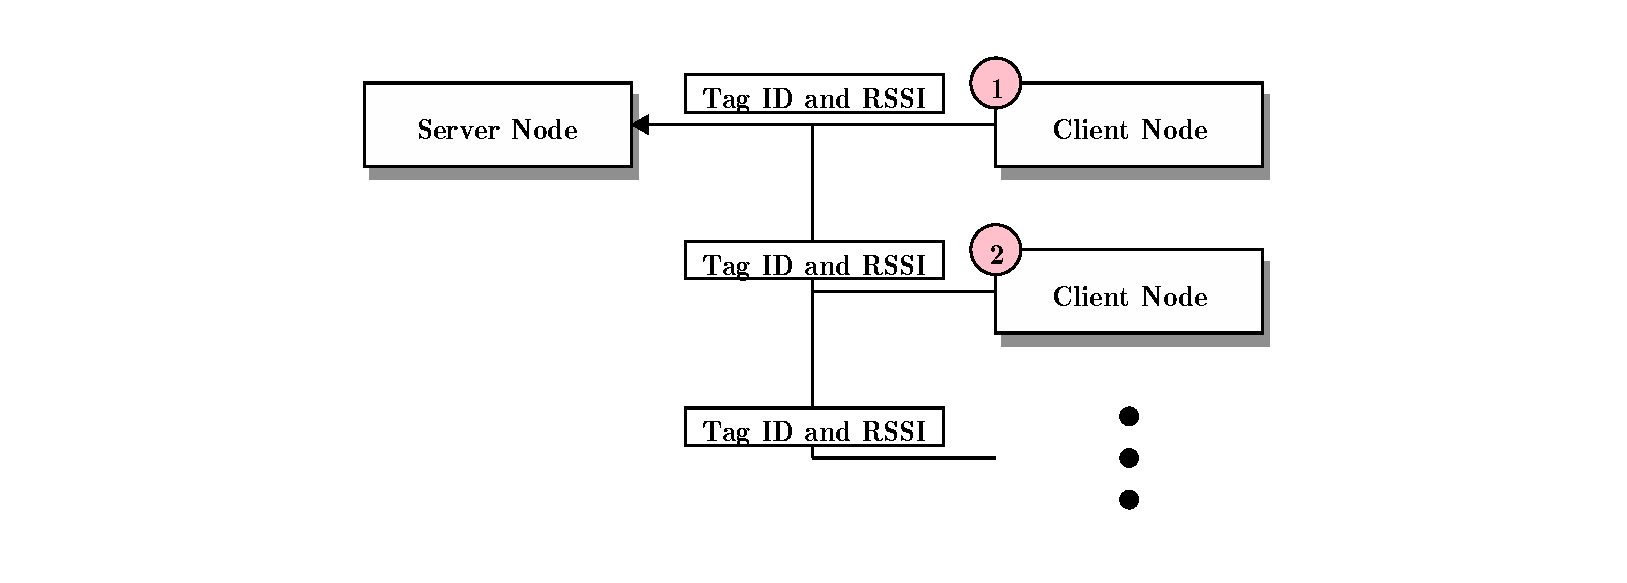
\includegraphics[width=1\textwidth]{figures/blockdiag/serverclient}
		\caption{Conceptual diagram of the server-client model.}
		\label{fig:sercli}
	\end{center}
\end{figure}

Client nodes have two main responsibilities. First, they read the identity and RSSI of the tag. Second, clients send this data on the network to the server. A server node provides the following functionality. It receives measurements from other nodes. A server also reads the tag's identity and RSSI. Then, this computer converts the RSSI values into distance. Distance measurements together with the positions of the reader nodes are input into a localisation algorithm. These steps are illustrated on Figure \ref{fig:sercliresp}.

\begin{figure}[h]
	\begin{center}
		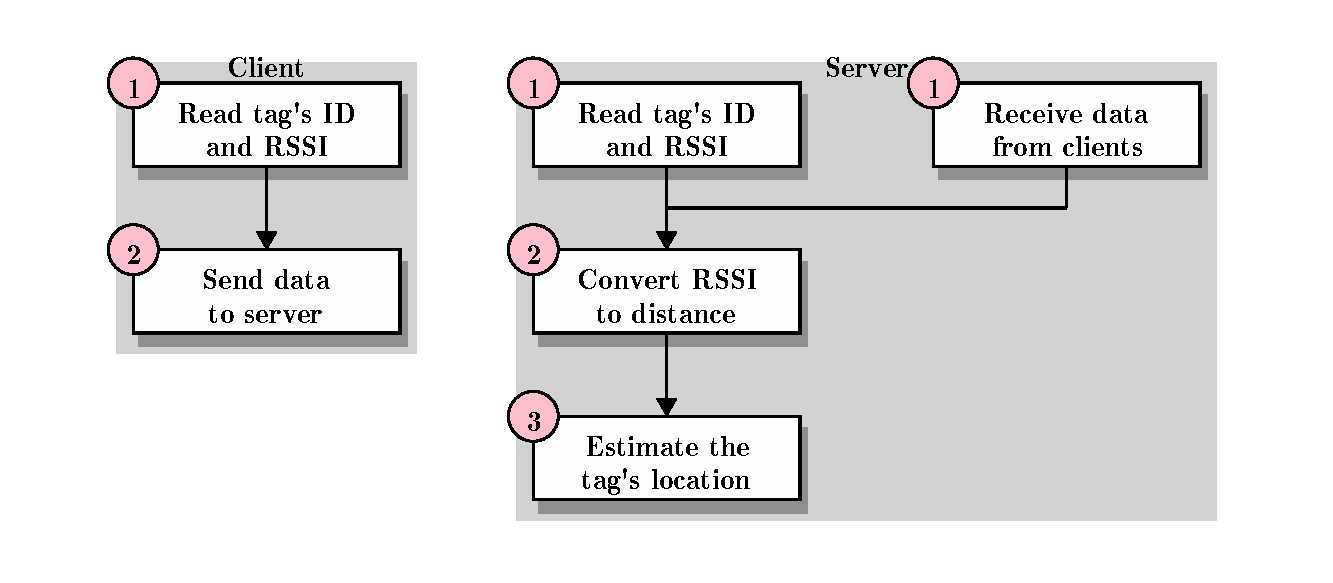
\includegraphics[width=1\textwidth]{figures/blockdiag/serverclientresp}
		\caption{Diagram of the general server and client responsibilities.}
		\label{fig:sercliresp}
	\end{center}
\end{figure}

\section{Converting RSSI to distance}
\label{sec:rssitodist}

One of the main challenges of this project was to find a reliable way of converting RSSI values into distance from RFID readers to a tag. As discussed in Section \ref{subsec:rsssianddist}, studies have shown that RSSI is not a reliable or accurate measure of distance. Nevertheless, RSSI is one of the main parameters of this system and distance estimation is solely based on it.

\subsection{Free-space Path Loss}

The first attempt to provide a conversion between RSSI and distance was relying on the inverse-square physical law and free-space path loss (FSPL) formula. In free space propagation, electromagnetic waves obey the inverse-square law stating that the intensity of the emitted radiation is inversely proportional to the square of the distance from the source of the emitted radiation \cite[p. 19]{Schlaikjer1962}. This can be expressed as the following relation:

\[ Intensity \propto \frac{1}{distance^{2}} \]

A more complete relationship between signal strength and distance is given by the FSPL formulation. Free-space path loss is the loss in signal strength of an electromagnetic wave propagating through free space without any obstacles \cite{Balanis2012}. FSPL is proportional to the square of both distance and frequency of the radio signal. It can be expressed in terms of decibels given distance in meters and radio frequency in megahertz\footnote{Derivation the dB version of the FSPL equation - \url{http://www.ece.uvic.ca/~peterd/35001/ass1a/node1.html}}: 

\[ FSPL(dB) = 20\log_{10}(d_{meters}) + 20\log_{10}(f_{MHz}) - 27.55 \]
	
Rearranging the terms of the equation to find the distance gives:

\[ d_{meters} = 10^{(FSPL(dB) - 20\log_{10}(f_{MHz}) + 27.55) / 20} \]

Section \ref{subsec:rssiandrss} discussed the relationship between RSSI and received signal strength (RSS). RSSI is a unitless measurement derived from the values of the RSS. In Section \ref{subsec:receiver}, Figure \ref{fig:rssi} shows the relationship between RSSI and RSS for the RFID receivers used in this project. Consequently, RSSI values can be converted to received signal strength expressed in $dBm$ and inserted into the equation above as $FSPL(dB)$. The frequency of the RFID project hardware is  $315MHz$ (see Table \ref{tbl:reader} and \ref{tbl:tag}).

There are three problems with this approach. First, it models how the signal strength decreases in a line-of-sight propagation in a free from obstacles environments. This project is concerned with location sensing in indoor spaces making the free-space path loss formula inappropriate for this setting. Second, computing the distance for the minimum ($0dB$) and maximum ($60dB$) values of the signal strength range results in distances $0.075$ and $75.716$ meters, which is beyond the practical range of the RFID devices. Third, the conversion from RSSI to RSS might not be appropriate in this case. The RFID equipment for this project is more affordable compared to commercial RFID equipment\footnote{How much do RFID readers cost today? - \url{http://www.rfidjournal.com/faq/show?86}}. As a result, the online support and specifications are scarce, which raises the question to what extent these can be trusted. Moreover, the manufacturer claims a RSSI resolution of eight bits outputting values between 0 and 255. During the range experiments with this hardware a much smaller resolution was recorded. Consequently, converting RSSI unitless values to received signal strength in $dBm$ cannot be relied upon. For details on the evaluation of the RFID devices refer to \textbf{REF}. 

\subsection{Translation table}

Rather than relying on the physical relationship between electromagnetic waves and distance, a simpler and more direct approach was taken. For each RFID reader, a translation table was constructed mapping RSSI to distance. According to the manufacturer, but also observed in hardware experiments, reader measurements vary between different devices. There are two reasons for this. First, the RFID readers are handmade, which introduces small differences in their circuits. Second, the devices are not calibrated to each other when being built.   

The methodology for constructing these translation tables relies entirely on RSSI measurements collected while evaluating the RFID devices. A number of experiments were conducted testing how RSSI changes as the distance between a reader and tag increases. In order to account for the characteristics of indoor environments, these experiments have taken into account the orientation of the tag to the reader, line-of-sight propagation versus obscuring the tag with an obstacle, and elevation of the tag to the reader. Combining measurements from different experiments gives a more realistic representation of how RSSI changes in an indoor environment. Table \ref{tbl:trans} presents the translation table constructed for the first reader. Similar tables were developed for the other two devices (see Appendix \ref{sec:trans}).

\begin{table}[h]
	\centering
	\begin{tabular}{ | c | c | c || c | c || c | c || c | c || c | c || c | c || c | c | }
		\hline
		Distance 	& 0  & 1  & 1  & 2  & 2  & 3  & 3  & 4  & 4  & 5  & 5  & 6  & 6  & 7  \\ \hline
		RSSI 		& 80 & 65 & 64 & 62 & 61 & 57 & 56 & 53 & 52 & 48 & 47 & 46 & 45 & 44  \\ \hline
	\end{tabular}
	\caption{RSSI value ranges used to estimate distance when using the first reader.}
	\label{tbl:trans}
\end{table}

As an example, the first two columns of Table \ref{tbl:trans} have the following meaning. When the reader and tag antennas were touching the average RSSI value from all experiments was 80. When the tag was one meter away from the reader, the average RSSI value of all experiment measurements was 65. RSSI values between 80 and 65 are linearly converted to the new range from zero to one meters as follows: 

\[Old.range = old.min - old.max \\\]
\[New.value = new.min + (old.min - old.value) / old.range\]

An obvious limitation of these conversions is the size of the RSSI ranges. For example, there are 15 possible values that the first reader could measure when the tag is between zero and one meters away from it. In contrast, for a distance between six and seven meters the RSSI values change only by one unit. Following from that, the granularity of the distance estimation changes depending on the range of the RSSI measurements. This is caused by a hardware limitation of the readers when measuring RSSI and has been found during the range experiments presented in \textbf{REF}.

There is another factor contributing to the accuracy of this conversion. The RFID tag is using a battery for its power supply. During continuous operation the battery power level gradually drops, thus the tag emits a weaker radio signal as the battery is being depleted. This is reflected in the RSSI measurements making the translation tables inaccurate. In order to account for the RSSI changes, the incoming measurements were increased by an integer factor chosen based on observation. Different factors were selected for each reader due to their measurement differences.

In summary, this conversion method is not universal and probably cannot be applied to other brands of RFID devices. There are numerous factors that contribute to the variations in RSSI such as radio signal reflection, multi-path fading, and shadowing, to name a few. Nevertheless, this method was selected to translate RSSI to distance. Once the translation tables are constructed, it is a matter of calibration. As mentioned above, RSSI to distance conversion is one of the main variables of this system. How these translation tables performed is discussed in Section \textbf{REF}, where the evaluation results of the system in terms of localisation accuracy are presented.


\section{Trilateration}
\label{sec:trilatmeth}

Trilateration is a localisation method computing the position of an unknown object based on range measurements from three reference points at known locations. The concept of this technique was described in Section \ref{sec:trilatback}. This section presents the mathematical technique used in this project that provides an exact and computationally efficient solution for three-dimensional position estimation. The solution is based on the work of Manolakis \cite{Manolakis1996} and the Wikipedia article on trilateration \cite{Wikipedi2013}.

\subsection{Special case}

In three-dimensional Cartesian coordinate system, the equations for three spheres are:
\begin{align*}
	r_1^2 &=(x-x_1)^2+(y-y_1)^2+(z-z_1)^2 \\
	r_2^2 &=(x-x_2)^2+(y-y_2)^2+(z-z_2)^2 \\
	r_3^2 &=(x-x_3)^2+(y-y_3)^2+(z-z_3)^2 \\
\end{align*}
where the sphere centres are $\vec p_1 = (x_1, y_1, z_1), \ \vec p_2 = (x_2, y_2, z_2), \ \vec p_3 = (x_3, y_3, z_3)$ and $r_1$, $r_2$, and $r_3$ are the sphere radii. Solving these equations for $x$, $y$, and $z$ would give their intersection point. However, this is hard to do directly. In order to simplify the calculations, a special case is defined that can be later used as the basis for a general solution. There are three requirements of the special case. First, the three centres of the spheres are on the $z=0$ plane, hence working in two dimensions. Second, one of the centres of the spheres, $\vec p_1$, is located at the origin. Third, another sphere centre, $\vec p_2$, is on the $x$-axis, thus two of the spheres are collinear. The equations for the three spheres can be rewritten as follows:
\begin{align}
	r_1^2 & =x^2+y^2+z^2 \label{eq:1}\\
	r_2^2 & =(x-d)^2+y^2+z^2 \label{eq:2}\\
	r_3^2 & =(x-i)^2+(y-j)^2+z^2 \label{eq:3}
\end{align}
where $d$ is the distance between sphere centres $\vec p_1$ and $\vec p_2$ and $i$ and $j$ are the signed magnitudes of the $x$ and $y$ components of the vector from $\vec p_1$ to $\vec p_3$. Figure \ref{fig:trilat2} illustrates these components and the positions of the spheres in the $z=0$ plane.

To solve these equations, first subtract \ref{eq:2} from \ref{eq:1} and solve for $x$:
\[x=\frac{r_1^2-r_2^2+d^2}{2d}\]
Next, subtract \ref{eq:3} from \ref{eq:1} and solve for $y$:
\[y=\frac{r_1^2-r_3^2+i^2+j^2}{2j}-\frac{i}{j}x\]
Finally, use \ref{eq:1} to solve for $z$:
\[z=\pm \sqrt{r_1^2-x^2-y^2}\]
These three equations  provide the coordinates of the intersection point $(x,y,z)$ of the three spheres.

\begin{figure}[h]
	\begin{center}
		\def\svgwidth{0.6\textwidth}
		\input{figures/trilat2.pdf_tex}
		\caption{Figure showing three intersecting spheres in the plane containing their centres. Figure from \cite{Wikipedi2013}.}
		\label{fig:trilat2}
	\end{center}
\end{figure}

\subsection{General solution}

The solution of the aforementioned case cannot be applied in a general three-dimensional case because its requirements are not met. This is overcome by treating the sphere centres, $\vec p_1$, $\vec p_2$, and $\vec p_3$, as vectors from the origin:
\begin{align*}
	\vec p_1 &= (x_1, y_1, z_1) \\
	\vec p_2 &= (x_2, y_2, z_2) = \vec p_1 + \hat e_x d \\
	\vec p_3 &= (x_3, y_3, z_3) = \vec p_1 + \hat e_x i + \hat e_y j \\
\end{align*}
where $\hat e_x$, $\hat e_y$, and $\hat e_z$ are the basis unit vectors in the $x$, $y$, and $z$ original coordinate system; $d$, $i$, and $j$ are the same variables defined above. The unit vectors and variables are expressed as follows:
\begin{align*}
	& d = \| \vec p_2 - \vec p_1 \|, &&  i = \hat e_x \cdot ( \vec p_3 - \vec p_1 ), && j = \hat e_y \cdot ( \vec p_3 - \vec p_1 ) \\
	& \hat e_x = \frac{ \vec p_2 - \vec p_1 }{ d }, && \hat e_y = \frac{ \vec p_3 - \vec p_1 - \hat e_x i}{ \| \vec p_3 - \vec p_1 - \hat e_x i \| }, && \hat e_z = \hat e_x \times \hat e_y
\end{align*}
Thus, the intersection point of the three spheres, which is the solution of the problem, is:
\[\vec p_{1,2} = \vec p_1 \ + \ \hat e_x x \ + \ \hat e_y y \ \pm \hat e_z z\]

This mathematical method is used to estimate the position of an RFID tag. It is efficient because trigonometric functions are not used. Instead, this method relies on elementary arithmetic operations \cite{Manolakis1996}. When implementing this method, one needs to account for some specific cases, for instance, when $d$ equals $0$. In this case, the sphere centres $\vec p_1$ and $\vec p_2$ share the same coordinates, which means that these two spheres are concentric. Consequently, no solution to the problem exists because these spheres cannot intersect when they have different radii and are the same sphere if they have equal radii. Section \textbf{REF} is concerned with the implementation details and conditions guarding for specific cases. 
